
The information from each subject was collected using a web-based form. To maintain anonymity, no personal information that could be used to trace the subject back was collected. The procedure used with each subject is described here below.

\begin{enumerate}
	
	\item The subject was asked to fill out the following information:
	
	\begin{itemize}
		\item Sex
		\item Job
		\item Age
		\item Country of origin.
	\end{itemize}
	
	\item The robot was shown to the participant and the experiment procedure explained.

	\item An example of the questionnaire was presented and a sample movement of the robot shown.

	\item The subject was exposed to a specific movement sequence according to the following steps:

	\begin{enumerate}

		\item The subject is exposed to the movement generated by a configuration of values.

		\item The subject could use as much time as needed to select values for intensity of the different terms in the questionnaire.

		\item After the subject had completed his/her selection about the current movement, the robot is positioned to the new starting point, and the sequence is repeated from step 1.(a) for the rest of movements.

	\end{enumerate}
\end{enumerate}

The order of the options enlisted in the questionnaire changed for each question to prevent any kind of bias. Figure~\ref{fig:questionnaire_example} shows an example of the questionnaire used. 

\begin{figure}
	\centering
	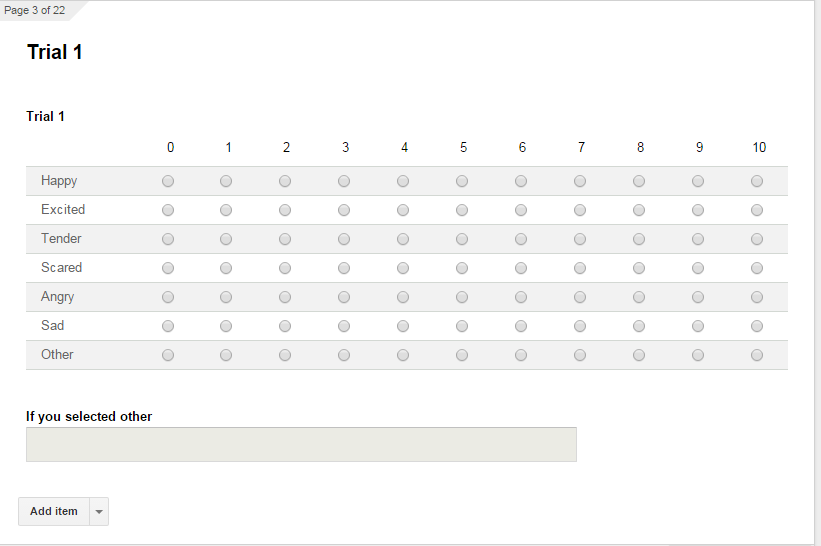
\includegraphics[width=0.48\textwidth]{./Images/example_survey.png} 
	\caption{Example of the questionnaire used in the experiment.}
	\label{fig:questionnaire_example}
\end{figure}

